\documentclass[a4paper,12pt]{scrartcl}
\usepackage[utf8x]{inputenc}
\usepackage[T1]{fontenc} % avec T1 comme option  d'encodage c'est ben mieux, surtout pour taper du français.
%\usepackage{lmodern,textcomp} % fortement conseillé pour les pdf. On peut mettre autre chose : kpfonts, fourier,...
\usepackage[french]{babel} %Sans ça les guillemets, amarchpo
\usepackage{amsmath}
\usepackage{multicol}
\usepackage{amssymb}
\usepackage{tkz-tab}
\usepackage{exercice_sheet} 



%\trait
%\section*{}
%\exo{}
%\question{}
%\subquestion{}

\date{}


% Title Page
\title{Devoir en classe, préformation Bac Pro Optique}

\author{\rotatebox{10}{\textsc{Géométrie}} \\ 40 minutes}

\begin{document}

\maketitle

{\Large Nom:} 
\hspace{60mm}
{\Large Prénom:}
\vspace{6mm}

Note : la calculatrice est autorisée. Donc sauf mention contraire, tout résultat donné sans la moindre étape de calcul ne sera pas pris en compte...

\exo{Rectangles}
On considère un rectangle de 8cm de large et 12cm de long.

\question{Donner le périmètre $\mathcal{P}_1$ et l'aire $\mathcal{A}_1$ de ce rectangle}
\lignes{1}

\question{Ce rectangle subit un agrandissement de facteur $k = 1.5$. Donner le périmètre $\mathcal{P}_2$ et l'aire $\mathcal{A}_2$ de ce nouveau rectangle} 
\lignes{2}

\exo{Triangles}

\begin{center}
\includegraphics[width=0.3\linewidth]{pics/triangle.png}
\end{center}

Le triangle $ABC$ a pour base $[AB]$, de longueur 8cm et pour hauteur $[HC]$, de longueur 4cm. 

\question{Quelle est la définition d'une hauteur dans un triangle?}
\lignes{2}

\question{Quelle est l'aire du triangle ABC ? Détailler les calculs.}
\lignes{2}

\question{Quelle est la définition d'une médiane dans un triangle?}
\lignes{2}

\exo{Quadrilatères}

Pour cet exercice, vous pourrez répondre soit par écrit soit en dessinant les codages sur les figures.

\question{Rappeler les propriétés d'un parallélogramme. }
\lignes{1}

\begin{center}
\includegraphics[width=0.3\linewidth]{pics/parallelogramme.png}
\end{center}

\question{Un losange est un parallélogramme particulier. Il hérite donc de ses propriétés, mais il en a en plus. Quelles son-elles?}
\lignes{1}

\begin{center}
\includegraphics[width=0.4\linewidth]{pics/losange.png}
\end{center}

\section*{Tracés}

Dans cette partie les tracés lorsqu'il y en a doivent être réalisés \fbox{\textbf{au compas}} et les traits de construction doivent être laissés.

\exo{Tracer la parallèle à la droite passant par le point C}

\begin{center}
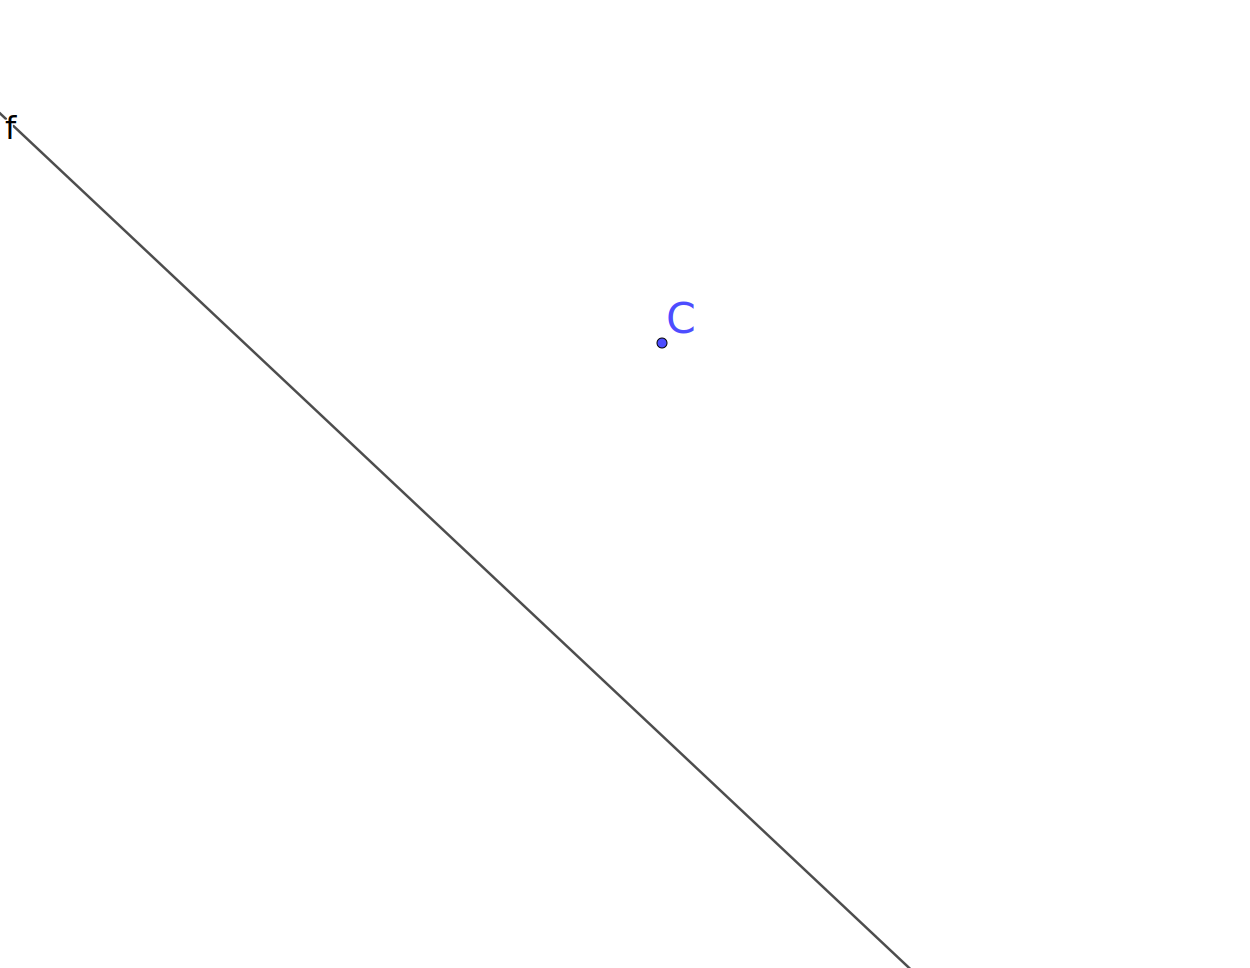
\includegraphics[width=0.8\linewidth]{pics/parallele_point.pdf}
\end{center}

\exo{Tracer la perpendiculaire à la droite passant par le point C}

\begin{center}
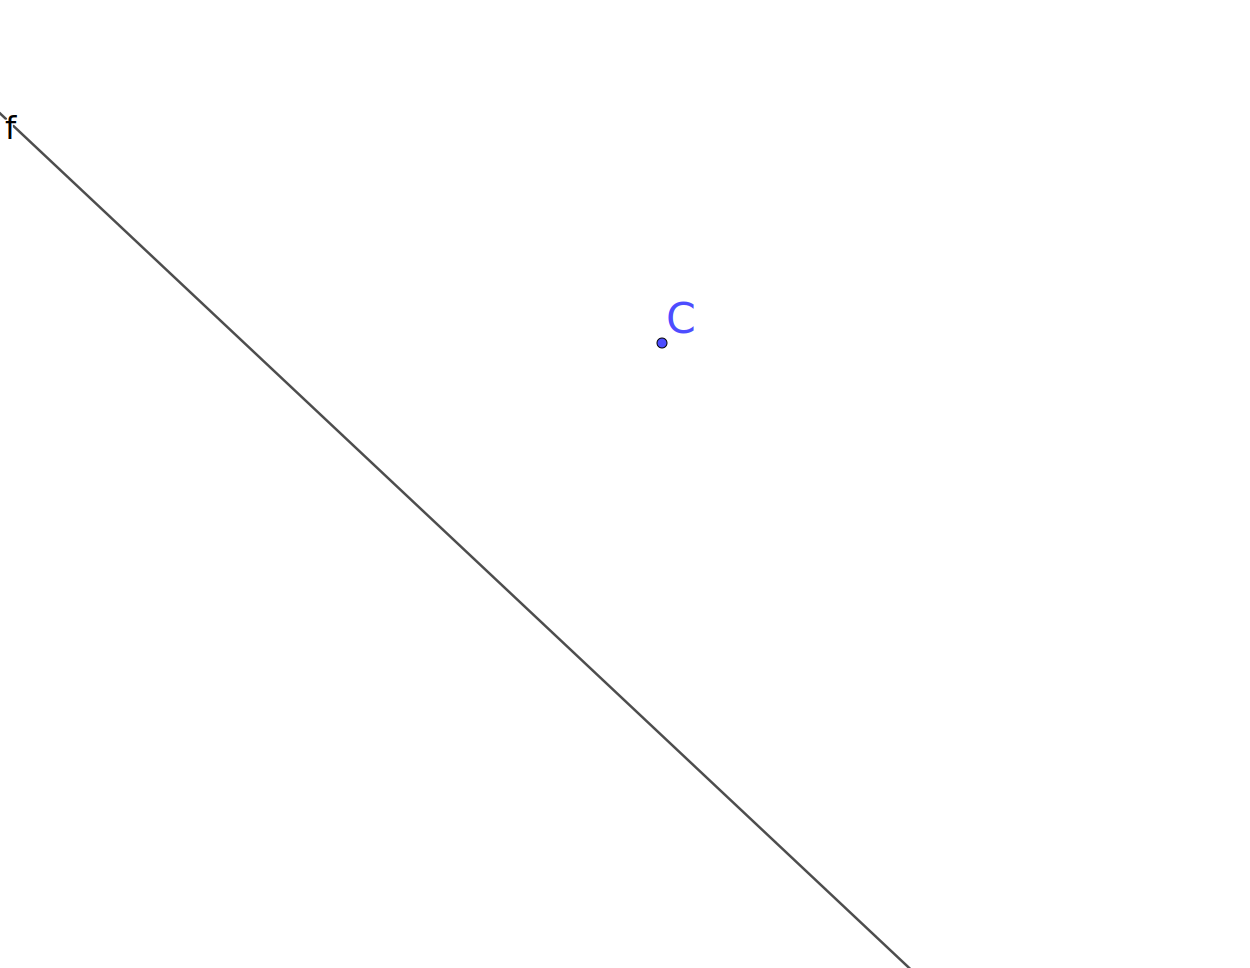
\includegraphics[width=0.8\linewidth]{pics/parallele_point.pdf}
\end{center}

\exo{Le théorème de Pythagore}

Un triangle $ABC$ est rectangle en A. Le côté [AB] mesure 3 cm et le côté [AC] mesure 4 cm. Quelle est la longueur du côté [BC] ?

\exo{La réciproque du théorème de Pythagore}

Soit un triangle $ABC$. Ses côtés on les longueurs données comme suit : 

\begin{itemize}
\item $[AB]$ a une longueur de 7 cm
\item $[AC]$ a une longueur de 12 cm
\item $[BC]$ a une longueur de 14 cm
\end{itemize}

Le triangle $ABC$ est-il rectangle ?

\trait

\begin{center}
Fin.
\end{center}

\end{document}

